% \section{Learning Pipeline}
% \label{learning_pipeline_section}
TODO 3*3 EXAMPLE TO HIGHLIGHT HOW EACH STEP WORKS

The overall pipeline is shown in Figure \ref{fig:pipeline}. By interacting with the environment, an agent accumulates state transition experiences as positive examples, which is used by ILASP to learn and improve hypothesis.
The agent also records surrounding information it has seen as background knowledge, which is used to make a plan together with the hypothesis that ILASP learns by solving an answer set program. 
Mechanisms of each step is explain in details in the following sections. 

\begin{figure}[!htb]
\centering
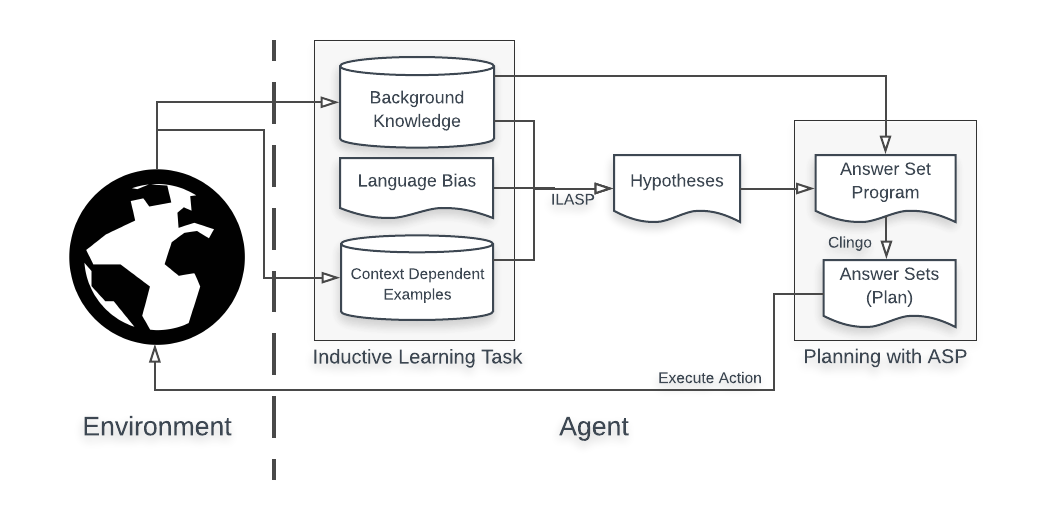
\includegraphics[width=0.8\textwidth]{./figures/architecture}
\caption{Reinforcement learning pipeline using ILASP. ILASP learns to generate a modelof the environment, or hypothesis, and updates it based on the interaction with the environment. }
\label{fig:pipeline}
\end{figure}

\section{Experience Accumulation}
\label{experience_accumulation}
\textcolor{red}{Draw an illustration of the difference between exploration and las part}\\
\textcolor{red}{Related these with Definition of ILASP}\\
The first step is to accumulate experience by interacting with the environment. Similar to tranditional RL agent, an agent explores an environment randomly until it reaches the goal once. 
Every time the agent takes an action during the exploration phase, these experiences need to be recorded in two different forms: \textit{state transition experience} and \textit{environment experience}.

\subsection{State Transition Experience}
\textit{State transition experience} contain information about how the state transition at each time step.
 It is the same as E\textsuperscript{+} in ILASP, especially positive examples for ILASP in ASP syntax, which is of the form:

\begin{equation}
\begin{split}
\textsf{\#pos(} & \textsf{\{state\_after((X2,Y2))\}},\\
& \{\textsf{all other state\_after that did not happen}\}, \\
& \{\textsf{state\_before((X1,Y1)). action(A). surrounding information}\}).
\end{split}
\end{equation}
where,
\begin{itemize}
    \item inclusions contain one state\_after((X2,Y2)), which represents the position of the agent in x and y axis after an action is taken 
    \item exclusions contain all other state\_after((X,Y)) that did not occur
    \item context example include state\_before((X1,Y1)), which represents the position of the agent in x and y axis before an action is taken,
    action(A) is the action the agent has taken, and surrounding information, such as walls, if any. 
\end{itemize}

These experience need to be expressed in ASP form in order to execute the inductive learning in ILASP. The input used in ILASP is state transitions, 
rewards and an action of the agent, 
% which can be directly converted using a simple mapping table or an action language (such as BC\textsuperscript{+} as used in \cite{Ferreira2017}). 

\textcolor{red}{exclusions are determined by the state that did not happen.}
The inclusions and exclusions are determined by the following algorithms
\begin{equation*}
\begin{split}
    &\forall s \in \textsf{State, agent is at s, ASP of H does not contains s as state\_after, add s} \rightarrow \textsf{INC.} \\
    & \forall s \in \textsf{State, agent is not at s, ASP of H contains s as state\_after, add s} \rightarrow \textsf{EXC.} 
\end{split}
\end{equation*}

Where INC and EXC are inclusions and exclusions respectively. ASP is Answer Set Program P and H is the current hypothesis. 
context example are
\begin{itemize}
    \item the state that the agent was before taking action (represented as \textit{state\_before(x,y)})
    \item an action that the agent takes (representend as \textit{action(a)})
    \item surrounding information of \textit{state\_before(x,y)}, such as walls. 
\end{itemize}

% \textcolor{red}{There is no negative example as XXXX.}

Using these positive examples, the agent is able to learn and improve hypothesis as it explore the environment and encounters new scenarios. 

\begin{examp} \normalfont (Positive examples). 

Suppose an agent takes an action "up" to move from (1,3) to (1,4) cell. All other alternative states that the agent could have ended up by taking different actions 
(down, right, and left) are in the exclusions. Finally surrounding walls information are in the context.

\begin{equation*}
\begin{split}
    \textsf{\#pos(} & \textsf{\{state\_after((1,3))\},}\\
                    & \textsf{\{state\_after((2,4)),state\_after((1,5)),state\_after((0,4)),state\_after((1,4))\},} \\
    & \textsf{\{state\_before((1,4)). action(up). wall((1, 5)). wall((0, 4)).\})}
\end{split}
\end{equation*}

This example will be used to learn how to move up as one of the agent's hypotheses.

Another example is 

\begin{equation*}
\begin{split}
\textsf{\#pos(} & \textsf{\{state\_after((1,3))}, \\ 
                & \textsf{\{state\_after((2,3)),state\_after((1,4)),state\_after((0,3)),state\_after((1,2))\}} \\       
                & \textsf{\{state\_before((1,3)). action(up). wall((2,3)). wall((0,3)). wall((1,2)).\}).}
\end{split}
\end{equation*}

where the agent tried to move up, from (1,3) to (1,2), but ended up in the same cell at (1,3). This is because there is a wall at (1,2), and the agent learns in order to move an above cell,
there must not be a wall in the above cell. 

\end{examp}
\label{state_transition_example}

\subsection{Environment Experience}

While the agent explores in the environment, it also remembers all the surrounding information as background knowledge, 
which will be stored in different repository, and are later used to generate a sequence of actions plan using H.

These experience correspond to B in ILASP definition. 

This does not include state transition experience, as these state\_before and action takens are different at every timestep.
Backgroud knowledge will be 

In static environment (e.g no moving enermy), environment information remain the same across time, and thus it will be beneficial to remember. 
This principle is different from most RL methods, as they are model-free learning. 
As described in XX,, model-based learning converge to optimal policy more efficiently. 

In a simple maze, these could be all wall position that the agent has seen so far, which can be 
wall((1, 5)). which represents the location of the wall. 
Another example could be a location of a teleportation if the agent sees it. 

These environment experiences are part of context examples in the positive examples. 

\section{Inductive Learning}
\label{induction}
Throughout the learning process, the agent accumulates positive examples and learn hypothesis H. 

Our learning task is XXX.

In order to execute ILASP, the following definitions are supplied as well as the positive examples,

\subsection{Search Space}
In order to execute ILASP, a \textit{search space} of possible hypotheses is required, which is defined using a \textit{language bias}. 

\begin{equation}
\begin{split}    
&\textsf{\#modeh(state\_after(var(cell))).}\\
&\textsf{\#modeb(1, adjacent(const(action), var(cell), var(cell))).} \\
&\textsf{\#modeb(1, state\_before(var(cell)), (positive)).} \\
&\textsf{\#modeb(1, action(const(action)),(positive)).} \\
&\textsf{\#modeb(1, wall(var(cell))).} \\
\end{split}
\end{equation}
Without these in the form of mode bias, the search space for ILASP will be empty. 


\begin{equation}
\begin{split}
&\textsf{cell((0..7, 0..6)).}\\
&\textsf{adjacent(right, (X+1,Y),(X,Y)) :- cell((X,Y)), cell((X+1,Y)).} \\
&\textsf{adjacent(left,(X,Y),  (X+1,Y)) :- cell((X,Y)), cell((X+1,Y)).} \\
&\textsf{adjacent(down, (X,Y+1),(X,Y)) :- cell((X,Y)), cell((X,Y+1)).} \\
&\textsf{adjacent(up,   (X,Y),  (X,Y+1)) :- cell((X,Y)), cell((X,Y+1)).} \\
\end{split}
\end{equation}

where \textit{var(t)} and \textit{const(t)} are a placeholder for variable and constant terms of type t respectively.


\textit{const(t)} must be specified as \#constant(t,c), where t is a type and c is a constant term. 
In our environment, action is specified as constant since ILASP should learn different hypothesis for each action.

\begin{equation}
\begin{split}
&\textsf{\#constant(action, right).}\\
&\textsf{\#constant(action, left).}\\
&\textsf{\#constant(action, down).}\\
&\textsf{\#constant(action, up).}\\
\end{split}
\end{equation}

As we describe in XXX, the search space increases in propotion to the complexity of learning tasks, which slows down the learning process.
For example, the search space in this particular setting is in XX. 

\#max\_penalty defines the maximum size of the hypothesis, by default it is 15. 
Increasing \#max\_penalty allows ILASP to learn longer hypothesis in expense of longer computation.
\#max\_penalty(50).

Together with the above defition as well as accumulated positive examples, ILASP is able to learn an hypothesis. The quality of H depends on the experiences for the agent. 
For example, In the early phase of learning, the agent does not have many examples, and learns an hypothesis that may not be insightfull. 
For example, if the agent has only one positive example, 

Next, the scope of \textit{cell} are defined, as cell((0..X, 0..Y)), where X and Y are size of width and height respectively.

Finally, since our learning task is the rule of the game, which involve state transition, it needs to know how it means to be "being next to XX",
Therefore the following assumptions are provided as background knowledge. 
\begin{equation}
\begin{split}
&\textsf{state\_after(V0) :- adjacent(right, V0, V1), state\_before(V1), action(right), not wall(V0).}\\
&\textsf{state\_after(V0) :- adjacent(left, V0, V1), state\_before(V1), action(left), not wall(V0).}\\
&\textsf{state\_after(V0) :- adjacent(down, V0, V1), state\_before(V1), action(down), not wall(V0).}\\
&\textsf{state\_after(V0) :- adjacent(up, V0, V1), state\_before(V1), action(up), not wall(V0).}
\end{split}
\end{equation}

This definition itself could be learnt by setting another learning tasks, and it is a potential learning problem. 
% TODO state represetation 
However, we focus on learning task of the rule of the game in this paper. 

The full details for ILASP learning tasks is described in Appendix XXX.
Positive excludes the possibility of negation as a failure in order to reduce the search space.

Future research will relax these assumptions and attemp to learn more general hypothesis, 
e.g learning adjacent defintion. 

These learnt H will be used to generate a plan in the abduction phase. 

After executing the plan, the agent will have more positive examples, which will be used to improve the quality of H. 

The learnt hypothesis is XXX

This hypothesis, for example, does not explain how to move "down". In order to learn how to move "down", it needs an positive example of moving up. 

later on H improving as we collect more examples as well as background knowledge.

\section{Plan Genreation}
\label{Plan_genreation}

Once the agent find the goal once, we can generate a plan using the current hypothesis by solving Answer Set Program. 

If the hypotheses were not accurate, clingo might not generate all the actions leading to the goals. 

The syntax of ASP is different from ILASP phase, because we need to include time sequence when solving ASP.
In ILASP, it is only state\_before and staet\_after, but in plan generation, there will be more than one state transition. 
% These conversion are done

\begin{equation}
\begin{split}
&\textsf{1\{action(down,T); action(up,T); action(right,T); action(left,T); action(non,T)\}1} \\
&\textsf{ :- time(T), not finished(T).}\\
\end{split}
\end{equation}

This choice rule states that action must be one of four actions (defined maximum and minimum numbers in 1), 
T is the time step at which the agent takes each action, unless \textit{finished(T)} is grounded. 

\textit{finished(T)} is associated with goal definition, and it is defined as:

\begin{equation}
\begin{split}
&\textsf{finished(T):- goal(T2), time(T), T} \geq \textsf{T2.}\\
&\textsf{goal(T):- state\_at((5, 1), T), not finished(T-1).}\\
&\textsf{goalMet:- goal(T).}\\
&\textsf{:- not goalMet.}
\end{split}
\end{equation}
    
\section{Plan Execution}
\label{Plan execution}

the plan generated by clingo is a set of states and actions. 

states are of the form state\_at((X,Y),T), where X and Y represent x-axi and y-axi in a maze respectively, T represents a time that the agent is at 
this particular X,Y cell. 

action(A,T) tells which action the agent should take at each time. By following the actions, the agent should collect both predicted state that the 
agent will end up, and the observed state that the agent actually end up. If there is a difference between these two, either B or H do not correctly represent
the model of the true environment, so needs to be improved. 

When the agent encounters a new environment (e.g a new wall), this new information will be added to its background, which will be used to improved the hypothesis 
next time ILASP gets executed. 

For example, 
\begin{equation*}
\begin{split}
&\textsf{state\_at((1,1),1), action(right,1)}\\
&\textsf{state\_at((2,1),2), action(right,2)}\\
&\textsf{state\_at((3,1),3), action(right,3)}\\
&\textsf{state\_at((4,1),4), action(right,4)}\\
&\textsf{state\_at((5,1),5)}, \cdots
\end{split}
\end{equation*}

At the start of the learning, H is usually not correct or too general, using this H will generate lots of answer sets that are not useful for the planning. 
These examples will be collected and included as exclusions of a new positive example. 

% For example, 
% XXX

To avoid the agent from being stuck in a sub-optimal plan, the agent deliberately discards the plan and takes an random action with a probability of 
epsilon (which is less than 1) TODO define this mathematically. 
When the agent deviates from the planning, it often discovers new information, which will be added to B.
Exploration is necessary to make sure that the agent might discovers a shorter path than the current plan, which will be demonstrated in the experiment. 

Define them here

ILP(RL) works by 

It buids the model of the environment by improving two internal concepts: hypothesis H and background knowledge B. 
% First, an agent explores an environment by taking random actions until it reaches the goal. 

In the further research, we could experiment with a more sophisticated exploration strategy, such as XXX and YYY. 

This is formally defined in Algorithm. 

\begin{algorithm}
\caption{ILP(RL)}\label{euclid}
\begin{algorithmic}[1]
\Procedure{ILP(RL) (B and E)}{}

\While {True}

    \State $\textit{H (inductive solutions)} \gets \text{run ILASP(T)}$
    \State $\textit{plan(actions, states) answer sets} \gets \text{AS(B, H)}$
    \While {actions in P}
        \State $\textit{observed state} \gets \text{run clingo(T)}$
        \If {$ \textit{observed state} \neq \textit{predicted state} $}
            \State $\textit{H} \gets \text{run ILASP(T)}$
            \EndIf
        % \If {$ \textit{observed state not equal \textit{predicted state $} 
        % \EndIf
    \EndWhile
    % \If {$ new \ background \ encountered $}
    %     % \State $\textit{H} \gets \text{run ILASP(T)}$
    % \EndIf
    % \For{i from 0 to N} 
    %     \If {$ A[i]\ is \ in \ T$}
    %         \State \Return $FALSE$
    %     \Else 
    %         \State Add A[i] to T   
    %     \EndIf
    % \EndFor
% \State \Return $TRUE$
\EndWhile

\EndProcedure
\caption{ILP(RL) }
\end{algorithmic}
\end{algorithm}

Everytime the agent executes an action by following the plan, it checks whether the observed state is that is expected. 

If there is a difference between the two, either

B is incorrect

H is not sophisticated enough, 

If that is the case, the agent runs ILASP again using more positive examples it collected during the plan execution. 

% \begin{itemize}
% \item States: XXX
% \item Actions: The agent can move up, down, right or left
% \item Rewards: XXX
% \item Transitions: XXX
% \end{itemize}

\section{Exploration}
\label{exploration}

ILP(RL) kicks in once the agent reaches a goal once. However it is likely that the agent has not seen all the environment
and therefore is likely to be in a sub-optimal plan. Therefore, similar to RL algorithm, the agent also has to explore a new state. 
There are a number of exploration strategy in RL (such as Boltzman approach, Count-based and Optimistic Initial value TODO REFERENCE). 
One of the most commonly used strategy is $\epsilon$-greedy strategy. As described in Chapter XXX, the agent takes an random action 

This strategy may not be appropriate in cases there safety is a priority (since it is random action.)
It is simple to implement. 
In the case of ILP(RL), the agent discard the plan from the abduction with a probably of epsilon and takes a random action in order to avoid getting stuck in a sub-optimal path. 
When the agent takes an random action and move into a new state, the agents creates a new plan from the new state and continue to move forward.

This exploration point will be highlighted in Experiment XXX.

Epsilon needs to be larger than Q-learnig because